% !TEX program = xelatex
% =====================================================================
% Overleaf 编译说明：
%   1) Overleaf 左上角 Menu -> Compiler 选 "XeLaTeX"（因含中文批注，用 xeCJK/Fandol）。
%   2) 需要的文件：main.tex, refs.bib, figures/fig1_pipeline.pdf,
%      figures/fig2_taxonomy.pdf, figures/fig3_filter_result.pdf。
%   3) 文献用 BibTeX（Overleaf 会自动跑）。
%   本地编译：latexmk -xelatex main.tex  （或 xelatex; bibtex; xelatex; xelatex）
% =====================================================================
\documentclass[11pt]{article}

\usepackage[fontset=fandol,scheme=plain]{ctex}   % 英文为主 + 少量中文批注（Fandol，随 TeXLive/Overleaf 自带）
\usepackage[margin=1in]{geometry}
\usepackage{amsmath,amssymb}
\usepackage{booktabs}
\usepackage{array}
\usepackage{multirow}
\usepackage{graphicx}
\usepackage{xcolor}
\usepackage{caption}
\usepackage{enumitem}
\usepackage[numbers]{natbib}
\usepackage{tikz}
\usepackage{pgfplots}
\pgfplotsset{compat=1.18}
\usepackage{microtype}
\usepackage[hidelinks]{hyperref}
\emergencystretch=3em   % 吸收长 \texttt 路径串导致的 overfull

\definecolor{accent}{HTML}{2563EB}
\definecolor{accdk}{HTML}{1D4ED8}
\definecolor{good}{HTML}{16A34A}
\definecolor{bad}{HTML}{DC2626}
\definecolor{barA}{HTML}{9AA3AF}

\newcommand{\code}[1]{\texttt{#1}}
\newcommand{\flag}[1]{{\color{bad}〔#1〕}}     % 红色醒目批注宏（定稿未使用；保留以防注释需要）

\setlist[itemize]{leftmargin=1.4em,topsep=2pt,itemsep=2pt}
\captionsetup{font=small}

\title{\textbf{Reachability, Not Discrimination: When Does Execution Grounding Help LLM Line-Level Fault Localization?}\\[2pt]
\large A Controlled Study of Self-Consistency and Coverage Signals}
\author{}
\date{}

\begin{document}
\maketitle
\vspace{-3.5em}

% =====================================================================
\begin{abstract}
\noindent
Resolving a real software issue with a large language model (LLM) requires first localizing the lines to edit within a repository far larger than any context window, and the \emph{recall} of this step upper-bounds repair: a faulty line that is never surfaced can never be fixed~\citep{liu_cannotfix,swebench}. In localize-then-edit pipelines the model reaches line-level candidates through its own test-time compute---sampling the code repeatedly and aggregating by \emph{self-consistency}~\citep{self_consistency}---but this internal signal plateaus with a characteristic shape: it surfaces a gold line into the top-10 (\emph{reachability}) far more often than it ranks it first (\emph{discrimination}). A recent wave of execution-grounded methods proposes to break the plateau by running the failing test and feeding its coverage/traceback/spectrum into the localizer, on the long-standing spectrum-based intuition that the code a failing test executes is where the bug lies~\citep{tarantula,ochiai,wong_survey}. Whether this external grounding actually adds what the model's own self-consistency cannot---discrimination---has not been tested at line granularity on real-world issues. We present a controlled study on SWE-bench-Lite that isolates the coverage effect by ranking the gold file's lines with and without execution information, so any difference is attributable to grounding rather than to the model or to file localization. We contribute three results. \emph{First}, we map the terrain: stratifying recall along six dimensions isolates file localization, gold-file size, and code domain as the dominant factors. \emph{Second}, we falsify execution coverage as a \emph{direct} signal: coverage is coarse (a median of 259 executed lines per gold file), structurally capped at 83\% recall on crash bugs because $\sim$16\% of fixes edit code that did not run, and its failing-versus-passing spectrum differential isolates the gold only for a control-flow-distinct minority (3 of the 9 instances where it is computable) and is empty for the rest. \emph{Third}, the one effective use of coverage is a recall-side \textbf{filter}: restricting candidates to executed lines, on the subset where the gold is on the executed path, raises line Recall@10 by 14 points while cutting the candidate set by 55\%---positive on all four backbones tested, significant on three. That on-path subset is \emph{gold-defined, an oracle routing}: without routing, the deployable always-filter floor is $+4.5$pp on all crash bugs, and a blind filter can be net-\emph{negative} on a backbone whose static off-path ranking is strong. And---like self-consistency---the filter lifts reachability, not discrimination: its Recall@1 change is not significant on \emph{any} of the four backbones, though on stronger backbones it does lift mid-rank Recall@5. A single distinction organizes all of it: execution coverage is a \emph{membership} (control-flow) signal, whereas SWE-bench faults appear predominantly \emph{data-level} (6 of 9 where directly measurable; a patch-structure proxy extrapolates a $\sim$66\% majority dataset-wide---indicative), so neither the model's self-consistency nor external coverage can rank the buggy line among its executed neighbours. Not every external signal helps an LLM equally: a signal that only certifies reachability cannot break a discrimination ceiling. (Richer execution signals such as mutation or value tracing, which could reach data-level faults, are out of scope.)
\end{abstract}

% =====================================================================
\section*{1.\quad Introduction}

To resolve a real software issue automatically, a large language model (LLM) must operate over an entire repository---reading the issue, navigating a codebase that spans thousands of files, and editing the code that fixes it~\citep{swebench,sweagent,agentless}. Whether the system is an end-to-end agent or an explicit localize-then-edit pipeline, it depends on \textbf{fault localization}---identifying the code units to change---and the \emph{recall} of this step is a hard upper bound on repair: a faulty line that localization never surfaces can never be patched, however capable the repair model~\citep{liu_cannotfix}. The bound is empirical, not merely formal: oracle-localization studies show that perfect localization lifts repair across systems, even as a substantial residual gap remains~\citep{beyondloc}.

File- and function-level localization are increasingly well handled. Graph- and retrieval-based agents reach file-level recall near 0.9~\citep{locagent,agentless}, and dedicated localization agents push function-level match rates higher still~\citep{orcaloca,cosil}. \emph{Line}-level localization---pinpointing the exact lines to edit---remains the weak link: even the strongest static line localizers report line-level recall well below their file- and function-level numbers~\citep{arise}. In a localize-then-edit pipeline the model narrows to lines through its own \emph{test-time compute}---sampling the numbered region $k$ times and aggregating by self-consistency~\citep{self_consistency,test_time_compute}---which is the workhorse of the pipeline but hits a ceiling of a particular shape: it reliably surfaces a gold line into the top-10 yet rarely ranks it first. Making matters worse, naively feeding more line-level context to the repair model can \emph{degrade} it through noise amplification~\citep{flcontext}; line localization must therefore improve \emph{recall} and \emph{precision} together, not merely widen the net.

A natural source of the missing signal is \textbf{execution}. Spectrum-based fault localization (SBFL) ranks statements by a suspiciousness coefficient over the failing-versus-passing coverage spectrum~\citep{tarantula,ochiai,dstar,wong_survey}, and dynamic slicing narrows attention to the statements that actually influence a failure on a given run~\citep{korel_laski,agrawal_horgan}; both are validated on crash-oriented benchmarks of isolated bugs such as Defects4J~\citep{defects4j}. A recent wave of execution-grounded LLM methods revives the idea, running the failing reproduction test and exposing its coverage or traceback to the model~\citep{autofl,autocoderover,agentfl}. The premise is that this external, execution-grounded signal supplies the discrimination the model's own sampling cannot. Yet the state-of-the-art line localizer is \emph{static}: ARISE augments the agent with a program graph and intra-procedural def-use slicing but never runs the code~\citep{arise}. This juxtaposition---a decades-old execution-based FL tradition, a static line-level SOTA, and an emerging assumption that execution should help---raises a sharp, untested question:

\begin{quote}
\textbf{When (if ever) does execution grounding help LLM line-level localization \emph{beyond} the model's own self-consistency, and how should it be used?}
\end{quote}

We answer it on SWE-bench-Lite with three research questions, each a self-contained empirical result. Our lens throughout is the distinction between two things an LLM localizer can gain: \emph{reachability} (getting a gold line into the top-$k$ candidate set) and \emph{discrimination} (ranking it first). We operationalize reachability as R@10---the a-priori primary endpoint (\S8)---and discrimination as R@1, with R@5 reported as an intermediate band (\S3.3). Self-consistency voting, the pipeline's own engine, buys reachability up to a ceiling; the question is whether external execution grounding can add the discrimination it lacks. We isolate the coverage effect by ranking the gold file's lines with the same static def-use score that underlies ARISE, with and without execution information, so that any difference is attributable to grounding rather than to the language model or to file localization.
\begin{itemize}
  \item \textbf{RQ1 (Terrain).} \emph{What depresses line-level recall, and by how much?} We stratify per-instance recall along six dimensions and identify file localization, gold-file size, and code domain as the dominant factors---the map on which the reachability ceiling sits (\S4).
  \item \textbf{RQ2 (Falsification + root cause).} \emph{Does execution coverage, used as a direct signal, add discrimination?} No. We give a mechanistic, falsifiable root cause spanning coverage coarseness, an 83\% structural recall ceiling, and a bug-dependent SBFL differential that is empty for the measured data-level majority (6/9; \S5).
  \item \textbf{RQ3 (The correct use).} \emph{Is there any effective use of execution coverage?} Yes---a recall-side \textbf{filter} (the role coverage already plays in agentic localizers such as AutoFL, here made explicit \emph{at line granularity} with on/off-path routing) that, on the on-path subset, raises reachability \emph{and} narrows the candidate set but---like self-consistency---does not add discrimination; every finer use fails, and we delimit the boundary (\S6).
\end{itemize}

\noindent\textbf{Contributions.}
\begin{enumerate}[leftmargin=1.6em,topsep=2pt,itemsep=2pt]
  \item \textbf{A characterization of why LLM line localization fails (RQ1).} A six-dimension stratification that quantifies the file-localization gate, a file-size precision wall, and a strong code-domain effect---factors that aggregate state-of-the-art numbers obscure.
  \item \textbf{A falsification of execution coverage as a direct line signal, with a mechanistic root cause (RQ2).} Coverage is coarse, structurally capped at 83\% recall on crash bugs by off-path fixes, and carries a failing-versus-passing differential that is bug-dependent (present only for control-flow-distinct faults, empty for the measured data-level majority, 6/9).
  \item \textbf{A coverage-as-filter method and a precise boundary (RQ3).} On the on-path crash subset the filter raises line Recall@10 by 14 points while cutting the candidate set by 55\%, replicated across four backbones (significant on three), resolving the recall/precision tension line-level context otherwise creates~\citep{flcontext}. The on-path contrast is \emph{oracle-routed}---the split is gold-defined---so it is the mechanism, not a deployable number; the un-routed deployable gain is $+4.5$pp, and a blind (un-routed) filter can be net-negative (\S6). Like self-consistency, the filter lifts \emph{reachability} (R@10) but not \emph{discrimination}: its R@1 gain is significant on none of the four backbones (Table~8); off-path it must be disabled, and every finer use (SBFL differential, slicing, region expansion) fails.
  \item \textbf{A unifying signal typology.} Both the model's own self-consistency and external execution coverage are \emph{membership} (control-flow) signals: they certify that a line is reachable but do not discriminate the buggy line from its executed neighbours, because SWE-bench faults appear predominantly \emph{data-level} (measured 6/9 where the spectrum differential is computable; a patch-structure proxy extrapolates $\sim$66\% dataset-wide---indicative, \S7). This single distinction organizes every negative result above---why coverage's \emph{score} term adds nothing, why the filter lifts R@10 but not R@1, why the SBFL differential is empty---and bounds \emph{coverage- and spectrum-based} line localization; richer execution signals (mutation, value/state tracing) that could reach data-level faults are out of scope (\S7).
\end{enumerate}

We deliberately scope this paper to \emph{characterizing and correctly using} execution grounding, and reserve the question of what signal breaks the discrimination ceiling (RQ4, \S9) for future work, so that the contribution holds independently of that harder goal.

% =====================================================================
\section*{2.\quad Background and Related Work}

\subsection*{2.1\quad LLM localization and repair on SWE-bench}
SWE-bench~\citep{swebench} casts repository repair as resolving a real GitHub issue so that hidden tests pass; its human-validated 500-instance subset SWE-bench Verified~\citep{swebench_verified} and the visual-domain SWE-bench Multimodal~\citep{swebench_mm} are now standard, though quality audits caution that a non-trivial fraction of ``solved'' instances leak the solution in the issue text or rely on weak tests~\citep{swebench_plus}. Two families of systems tackle the task. \emph{End-to-end agents} interleave navigation, editing, and test execution: SWE-agent equips the model with an agent--computer interface~\citep{sweagent}, AutoCodeRover performs structure-aware code search and optionally sharpens it with SBFL when a test suite is available~\citep{autocoderover}, and SpecRover adds specification inference~\citep{specrover}; a recent survey catalogs the resulting leaderboard architectures~\citep{dissecting}. \emph{Localize-then-edit} pipelines instead make localization explicit: Agentless uses a hierarchical file\,$\rightarrow$\,element\,$\rightarrow$\,line funnel over lexical and structural similarity~\citep{agentless}; LocAgent performs multi-hop search over a heterogeneous dependency graph, reaching file-level localization accuracy up to 92.7\% (it reports file/module/function granularities, not line)~\citep{locagent}; and OrcaLoca~\citep{orcaloca} and CoSIL~\citep{cosil} optimize function-level localization with agentic scheduling and code-graph search. Most relevant to us, \emph{ARISE}~\citep{arise} is the current \emph{line}-level state of the art: it extends a repository graph down to statement-level nodes connected by intra-procedural definition--use edges and exposes \emph{data-flow slicing} as a queryable agent tool, and reports the strongest line-level recall to date on SWE-bench-Lite with Qwen2.5-Coder-32B~\citep{qwen25coder}. Crucially, ARISE's signal is \emph{static}---it models how values \emph{could} flow, never how they \emph{do} flow at run time. Our base ranker is an independent reimplementation of the same def-use relevance score; on our end-to-end SWE-bench-Lite run it reaches an aggregate line Recall@\{1,5,10\}$=$29/43/47 (Table~1). We do not reproduce ARISE's reported numbers and make no absolute comparison to them; we use this ranker strictly as an \emph{internal} no-execution baseline and report only paired with/without-coverage contrasts on identical inputs. This isolates exactly one variable: whether adding \emph{execution} coverage to such a static def-use localizer supplies discrimination it lacks. (We additionally use the frontier model DeepSeek-V3~\citep{deepseekv3} in our characterization.)

\subsection*{2.2\quad Spectrum-based and dynamic fault localization}
The hope that execution helps localization has deep roots. SBFL ranks program elements by a suspiciousness coefficient over the passing/failing coverage spectrum---Tarantula~\citep{tarantula}, Ochiai~\citep{ochiai}, and D$^\ast$~\citep{dstar}, surveyed comprehensively in~\citep{wong_survey}. Mutation-based fault localization sharpens the signal by \emph{perturbing} the program and re-running the tests, ranking a location by how its mutants change pass/fail outcomes~\citep{muse,metallaxis}. Dynamic program slicing~\citep{korel_laski,agrawal_horgan} restricts attention to the statements that, on the observed execution, actually influence the value at a failure point. These techniques are the standard on benchmarks of \emph{isolated}, crash-oriented bugs with rich test suites such as Defects4J~\citep{defects4j}. A theme we return to: their discriminative \emph{ranking} power comes from counterfactual or dependence information (mutation, control- and data-dependence), not from raw coverage membership alone.

\subsection*{2.3\quad Execution signals, self-consistency, and verification in LLM-era localization}
LLM fault localizers increasingly consume execution. AutoFL~\citep{autofl} gives the model tools to fetch the classes and methods \emph{covered by the failing test} and then reasons over that narrowed set---using coverage to \emph{filter} the search space while the LLM does the ranking. AgentFL~\citep{agentfl} similarly tracks test behavior to scale fault localization to project-level context, and end-to-end repair agents run reproduced tests to \emph{validate} candidate patches~\citep{autocoderover,sweagent}. Across these systems execution serves two roles---bounding the candidate set, or checking a patch---rather than directly ordering lines by suspiciousness. Orthogonally, the ranking itself is typically produced by \emph{self-consistency}: sampling the model repeatedly and aggregating, a form of test-time compute that trades inference for accuracy~\citep{self_consistency,test_time_compute}. Self-consistency and self-verification have a known limit, however---a generator is often a poor verifier of its own outputs, and LLMs struggle to self-correct reasoning without an external signal~\citep{llm_as_judge,cannot_self_correct}, which is precisely why training an \emph{external} verifier helps on reasoning tasks~\citep{verifiers}. Our study connects these threads: we ask whether \emph{execution grounding} is the external signal that adds the discrimination self-consistency lacks, make the filter-versus-ranking distinction explicit, and test it head-on at line granularity on SWE-bench, where the faults differ markedly from Defects4J's.

\subsection*{2.4\quad Localization as the bottleneck, and the line-level tension}
That localization recall bounds repair is established pre-LLM: Liu et al.\ show that automated-program-repair results are biased and capped by which bugs fault localization can even find---``you cannot fix what you cannot find''~\citep{liu_cannotfix}. In the LLM era the bound is being re-examined: counterfactual upper-bound analyses quantify each localization stage's contribution to repair~\citep{rgfl}, and oracle-localization studies confirm that perfect localization lifts every system while leaving a residual frontier~\citep{beyondloc}. At the same time, finer localization is not automatically better---feeding line-level \emph{context} to a repair model frequently degrades it through noise amplification~\citep{flcontext}. This is precisely the tension our coverage-as-filter result resolves: it raises line-level recall while \emph{shrinking} the candidate set, improving recall and precision together.

\subsection*{2.5\quad Gap}
Prior work either assumes execution helps localization (the SBFL lineage) or, at the line level, avoids execution entirely (Agentless, LocAgent, ARISE); where LLM systems do use execution, they use it as an unexamined filter or a patch validator. No prior work tests, \emph{at line granularity on real-world issues, when execution coverage helps line localization and why}. We fill this gap, and trace every result to a single control-flow-versus-data-level distinction.

% =====================================================================
\section*{3.\quad Study Design}

\subsection*{3.1\quad Benchmark and gold convention}
We use \textbf{SWE-bench-Lite} (300 real instances; 100\% single-gold-file, matching the ARISE evaluation set). The gold edit lines are parsed from each instance's reference patch. To match the ARISE gold convention we drop blank-line and comment-only anchor lines (so we compare on the same target set; this is a fairness alignment, not a method choice). For the realism axis (\S4) we additionally use prior frontier-model runs on \textbf{SWE-bench Verified} (single-file, two-stage, and multi-file settings).

\subsection*{3.2\quad Base line-localization pipeline}
Our base pipeline (\code{region\_loc.py}) has four stages: (1) \textbf{agentic file localization} $\rightarrow$ candidate files; (2) \textbf{region narrowing}---show the LLM the file \emph{skeleton} (signatures + line ranges, $\sim$10\% of the file) and select suspect functions/classes, backstopped by graph- and coverage-ranked functions, turning ``find the line in 2000 LoC'' into ``find it in $\sim$200 LoC''; (3) \textbf{self-consistency vote}---numbered view of the region, $k$ samples, union by reciprocal-rank fusion (RRF); (4) \textbf{RRF ranking} over a def-use graph relevance score (\code{code\_graph.line\_scores\_v2}). Two backbones appear: Qwen2.5-Coder-32B and DeepSeek-V3.

\begin{figure}[t]
\centering
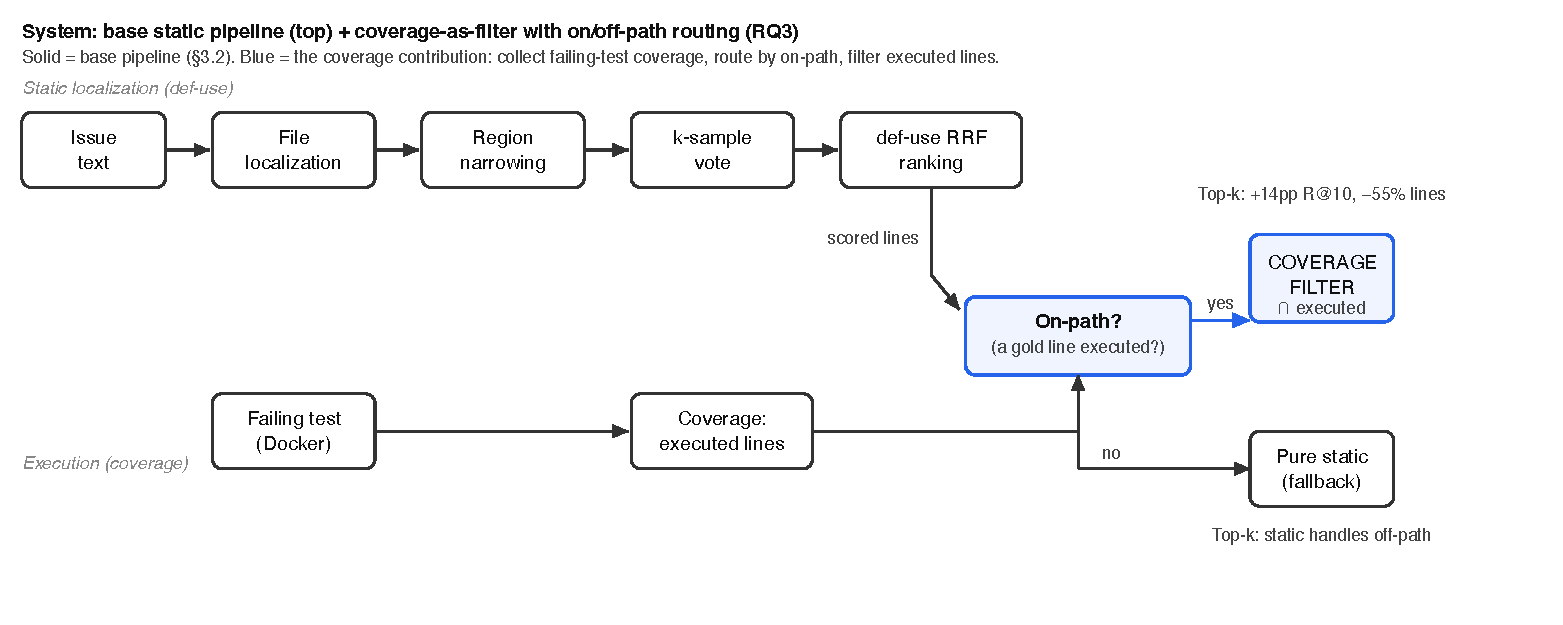
\includegraphics[width=\linewidth]{figures/fig1_pipeline.pdf}
\caption*{\textbf{Figure 1.} System overview. The base static pipeline (top lane, \S3.2) produces scored candidate lines; the execution lane (bottom) collects failing-test coverage. The \textbf{coverage contribution (blue, RQ3)} routes by \emph{on-path} (does any gold line appear in coverage?---an oracle split; a gold-free detector is future work, \S6): on-path, candidates are filtered to executed lines (+14pp R@10 offline / +12.3pp in the full pipeline, $-$55\% candidate lines); off-path, the filter would delete the gold, so the system falls back to pure static ranking.}
\end{figure}

\subsection*{3.3\quad Metrics}
\begin{itemize}
  \item \textbf{Line Recall@$k$} (the ARISE convention): an instance counts as a hit at $k$ if the top-$k$ predicted lines contain $\ge$1 gold line; we report $k\in\{1,5,10\}$.
  \item \textbf{MRR}: mean of 1/(rank of the first gold line), measuring how early the gold is found \emph{in absolute terms}.
  \item \textbf{Candidate-set size} (over-prediction width): the number of lines the ranker scores/predicts---our measure of ``net width'' for the wide-net precision problem.
  \item \textbf{Line-recall-given-found-file}: line recall conditioned on the gold file being found, isolating the line step from file localization.
  \item \textbf{Fraction recall}: the share of \emph{all} gold lines recovered (matters for multi-line fixes).
\end{itemize}
Throughout, we operationalize \emph{reachability} as R@10 (the a-priori primary endpoint, \S8) and \emph{discrimination} as R@1 (``ranks it first''); R@5 is an intermediate band reported as a secondary endpoint. Claims about discrimination are claims about R@1 under this operationalization.
To measure the \emph{coverage effect cleanly}, the RQ2/RQ3 ranking experiments are \textbf{file-given} (rank the gold file's lines): the def-use-only experiments (RQ2.2--RQ3.3) drop the LLM to isolate the coverage signal from file localization and from LLM variance, and RQ3.5 then confirms the headline filter effect inside the \emph{full} vote+graph+LLM pipeline on the same crash on-path subset.

\subsection*{3.4\quad Execution-data collection}
Coverage is collected inside the official SWE-bench Docker image per instance (\code{cov\_collect.py}): the test patch is applied and the failing test(s) are run under \code{coverage}, repo-aware (Django's \code{runtests.py} vs.\ pytest). For SBFL we additionally collect, per instance and in the same image, the \textbf{PASS\_TO\_PASS} coverage and the \textbf{isolated FAIL\_TO\_PASS} coverage (\code{rq3/cov\_collect\_pass.py}), enabling the failing-vs-passing differential. \emph{Collection limitation:} Django is skipped for SBFL (its \code{PASS\_TO\_PASS} names are not in pytest \code{file::test} form), and a collection attempt on three SymPy instances returned \emph{empty} coverage under the same harness and is excluded as no-data (not counted toward any denominator); the computable failing-vs-passing differential therefore spans $n{=}9$ instances over astropy, matplotlib, scikit-learn, seaborn (Table~3).

\subsection*{3.5\quad Bug-type classification and on-path scoping}
We label an instance \textbf{crash} if its issue text contains an explicit Python traceback or its added test asserts an exception (\code{pytest.raises}/\code{assertRaises}), else \textbf{behavioral} (\code{rq2/crash\_coverage\_analysis.py}; regex proxy, since validated against real FAIL\_TO\_PASS Docker runs---on/off-path agreed 68/68 with zero flips, \S8). Within crash, an instance is \textbf{on-path} if $\ge$1 gold line is in the failing test's coverage, else \textbf{off-path}. The four resulting subsets (crash/behavioral $\times$ on/off-path) are the unit of RQ3 analysis.

\smallskip\noindent\textbf{Subset bookkeeping (counts differ by collection).} Crash/behavioral counts are not identical across sections because the analyses draw on different coverage collections (\S3.4); within each, every reported number is internally consistent. RQ1 (\S4) labels all 300 Lite instances; the RQ2 coverage-coarseness statistics (\S5.2) are computed over instances whose gold-file coverage was collected by \code{crash\_coverage\_analysis.py}; and the recall-ceiling and RQ3/RQ4 ranking analyses (\S5.3,\,\S6) use the \emph{frozen} subset (\code{rq4/frozen\_subsets.json}), which additionally requires the gold \code{.py} file to expose a usable region with a computable gold$\cap$coverage ($n_{\text{cov-missing}}{=}50$). Hence the crash denominator is 77 in \S4/\S5.2 and 68 in \S5.3/\S6, and ``fraction of crash with a gold line executed'' reads 85.7\% (66/77, \S5.2) versus 83\% (57/68, \S5.3)---both correct for their population. The load-bearing crash on-path set is $n{=}57$ throughout (\S6, Table~4, Table~7). (The behavioral frozen set is $132$ on-path $+\,40$ off-path $=172$; one on-path behavioral instance lacks an evaluable def-use ranking and is dropped in the offline Table~4, giving $131$ there.)

\begin{center}\footnotesize
\begin{tabular}{lrrl}
\toprule
Analysis & crash & behav. & inclusion basis \\
\midrule
RQ1 (\S4, Table 1) & 77 & 223 & all SWE-bench-Lite (\code{is\_crash} label) \\
RQ2.1 prevalence & 70\,/\,89 & --- & traceback-strict\,/\,$+$raises-loose \\
RQ2.2 coverage (\S5.2) & 77 & 154 & $+$ gold-file coverage collected \\
RQ2.4 SBFL differential (Table 3) & 9 & --- & $+$ non-empty isolated F2P \emph{and} P2P coverage (\S3.4) \\
RQ2.3 ceiling, RQ3/RQ4 (\S5.3,\,\S6) & 68 & 172 & $+$ usable gold region, gold$\cap$cov (frozen) \\
\bottomrule
\end{tabular}
\end{center}

% =====================================================================
\section*{4.\quad RQ1 --- What depresses line-level localization recall?}

\noindent\textbf{Setup.} Before asking whether execution grounding adds discrimination (\S5--\S6), we map the terrain: \emph{where} recall is lost in the first place. We stratify per-instance end-to-end line recall on Qwen2.5-Coder-32B ($n$=300, SWE-bench-Lite, \code{rq1/rq1\_dimensions.py}) along six dimensions, reporting both line R@10 (end-to-end) and line-recall-given-found-file (the isolated line step) so we can separate file-localization effects from line-ranking effects. ARISE reports only aggregate localization metrics, with no per-repository, per-file-size, or per-bug-type breakdown~\citep{arise}; such a stratification at \emph{line} granularity is rarely reported.

\begin{table}[t]
\centering\small
\caption*{\textbf{Table 1 --- Stratified line recall (Qwen2.5-Coder-32B, $n$=300).}}
\setlength{\tabcolsep}{6pt}
\begin{tabular}{llrrrr}
\toprule
Dimension & Stratum & $n$ & line R@10 & rec\,$|$\,found & file-found \\
\midrule
\multirow{2}{*}{File found} & found & 221 & \textbf{63.3\%} & 56.1\% & 100\% \\
 & not found & 79 & \textbf{0.0\%} & 0.0\% & 0\% \\
\cmidrule(lr){1-6}
\multirow{4}{*}{Gold-file size (LoC)} & $\le$200 & 39 & 51.3\% & 44.3\% & 74\% \\
 & 200--1000 & 128 & 50.8\% & 43.8\% & 71\% \\
 & 1000--3000 & 116 & 43.1\% & 40.1\% & 76\% \\
 & $>$3000 & 17 & \textbf{29.4\%} & \textbf{24.3\%} & 76\% \\
\cmidrule(lr){1-6}
\multirow{2}{*}{\#gold lines} & 2--3 & 134 & 42.5\% & 45.1\% & 77\% \\
 & $\ge$4 & 166 & 50.0\% & \textbf{38.3\%} & 71\% \\
\cmidrule(lr){1-6}
\multirow{2}{*}{Bug type} & crash & 77 & 46.8\% & 43.5\% & 74\% \\
 & behavioral & 223 & 46.6\% & 40.6\% & 74\% \\
\cmidrule(lr){1-6}
\multirow{6}{*}{Domain (top repos)} & django & 114 & 54.4\% & 50.2\% & 77\% \\
 & sphinx & 16 & 56.2\% & 46.5\% & 75\% \\
 & sympy & 77 & 40.3\% & 33.2\% & 79\% \\
 & pytest & 17 & 41.2\% & 47.2\% & 59\% \\
 & matplotlib & 23 & 30.4\% & 25.8\% & 70\% \\
 & scikit-learn & 23 & \textbf{26.1\%} & 24.6\% & 43\% \\
\bottomrule
\end{tabular}
\end{table}

\begin{table}[t]
\centering\small
\caption*{\textbf{Table 2 --- Realism / task-complexity axis (illustrative).} A frontier LLM (DeepSeek-V3~\citep{deepseekv3}) on SWE-bench Verified, from a separate earlier run; included to show how the file-localization gate tightens with task complexity, \emph{not} for comparison with the Qwen2.5-Coder experiments elsewhere in the paper. Full provenance---model access, instance selection, prompts, and definitions of the ``(exact)'', ``e2e/given-found'', and ``over-prediction'' notations---is in Appendix~B; per-instance records ship in the artifact (\code{archive/p\{0,1,2\}\_openai\_deepseek\_v3.json}).}
\setlength{\tabcolsep}{6pt}
\begin{tabular}{lrll}
\toprule
Setting & $n$ & line recall & secondary obstacle \\
\midrule
single-file, file given & 40 & \textbf{0.584} (exact) & over-prediction 2.85$\times$ \\
realistic two-stage (find file + lines) & 40 & \textbf{0.528} e2e / 0.587 given-found & file hit@5 0.90 \\
multi-file (mean 2.45 gold files) & 20 & \textbf{0.277} global & \textbf{all-gold-files-found only 0.35} \\
\bottomrule
\end{tabular}
\end{table}

\noindent\textbf{Analysis.}
\begin{itemize}
  \item \textbf{(i) File localization is the dominant gate.} End-to-end line recall is 63.3\% when the file is found and \emph{exactly 0\%} otherwise; only 74\% of single-file instances ever reach the gold file. In the multi-file setting (Table 2) the gate tightens further: all gold files are found only 35\% of the time, and this file gate is the dominant driver of the collapse to 0.277 global line recall (Appendix~B). \emph{Line ranking cannot help an instance whose file is missed}---file localization is the first-order bottleneck.
  \item \textbf{(ii) File size is a precision wall, even given the file.} Line R@10 declines monotonically 51.3\%$\rightarrow$50.8\%$\rightarrow$43.1\%$\rightarrow$29.4\% with file size, and the \emph{given-found} column falls 44.3\%$\rightarrow$24.3\%---so the wall is in the line step itself, not just file localization. This is the quantified ``find the line in a big file'' problem.
  \item \textbf{(iii) Domain complexity is a strong, under-reported factor.} Numerical/scientific libraries (scikit-learn 26.1\%, matplotlib 30.4\%, sympy 40.3\%) are far harder than web/framework code (django 54.4\%, sphinx 56.2\%). scikit-learn additionally suffers a low file-found rate (43\%).
  \item \textbf{(iv) Multi-line fixes hurt fraction recall.} As \#gold-lines grows, \emph{given-found} recall falls 45.1\%$\rightarrow$38.3\%---recovering \emph{all} gold lines of a multi-line fix is harder, even though hitting \emph{one} (R@10) does not.
  \item \textbf{(v) Bug type does not affect achievable recall.} Crash (46.8\%) $\approx$ behavioral (46.6\%). This is important for RQ2/RQ3: bug type changes \emph{how} execution can help, not \emph{whether} a line is localizable.
\end{itemize}

% =====================================================================
\section*{5.\quad RQ2 --- Execution coverage is not a direct line-localization signal}

We build the falsification in four steps, each narrowing where execution could still help: crash bugs are the only place coverage could \emph{in principle} help, and they are a minority (RQ2.1); even there, raw coverage is a coarse, undiscriminating haystack (RQ2.2); worse, $\sim$16\% of crash fixes edit code that never ran, capping \emph{any} execution method at 83\% recall (RQ2.3); and the failing-vs-passing SBFL differential that might rank the rest is empty for the data-level cases, which dominate the instances we can measure (RQ2.4). All four collapse to one root cause (RQ2.5).

\subsection*{RQ2.1\quad Bug-type prevalence}
23\% of Lite instances contain an explicit traceback (crash-strict), 29\% when also counting tests that assert an exception (crash-loose)---$\approx$70--89 instances. Crash prevalence varies sharply by repo: astropy 66\%, matplotlib 60\%, seaborn 50\%, scikit-learn 43\%, sympy 37\%; vs.\ django 19\%, pytest 11\%, sphinx 0\% (\code{rq2/crash\_coverage\_analysis.py}). Crash bugs are where execution \emph{could} in principle help, so RQ2/RQ3 focus there.

\subsection*{RQ2.2\quad Coverage is coarse and barely bug-type-specific}
\emph{Granting that crash bugs exist, is raw coverage itself a usable candidate set? No.} The gold line is executed (instance-level, $\ge$1 gold line covered) for 85.7\% of crash (66/77; see the subset table in \S3.5) vs.\ 79.2\% of behavioral instances---a mere \textbf{+6.5pp}---while the executed set is a \textbf{median of 259 lines} per gold file (crash) vs.\ 279 (behavioral). Per-line gold-execution rate is 54.1\% (crash) vs.\ 47.0\% (behavioral). As a \emph{direct} candidate set, coverage is therefore a $\sim$259-line haystack with no internal ranking and almost no crash-vs-behavioral discrimination---reproducing and sharpening, at line granularity, the prior ``execution-as-direct-signal is falsified'' result.

\subsection*{RQ2.3\quad An 83\% structural recall ceiling---and why}
\emph{Even the coverage we do have has a hard ceiling.} On crash instances, only \textbf{83\%} (57/68) have \emph{any} gold line executed. We classify the 16\% gap (11 instances; \code{rq3/classify\_offpath.py}): \textbf{6 are off-path ``missed-branch''} fixes---the buggy run took the \emph{wrong} branch, so the fix line on the intended branch never executed---\textbf{4 are pure insertions} (added code that could not have run), and \textbf{1 is a function never reached}. Therefore:

\begin{quote}
\textbf{Execution coverage is structurally blind to fixes that target code which \emph{should have run but did not} (a missed branch) or \emph{does not yet exist} (an insertion).} No execution-based method---coverage, SBFL, or slicing---can recover such gold lines, capping coverage's line-recall at $\sim$83\% on crash bugs.
\end{quote}

\emph{Worked example (off-path missed-branch, django-14017).} The fix relaxes a branch condition in \code{Q.\_\_and\_\_} (\code{query\_utils.py}) from \code{if not isinstance(other, Q):} to also accept conditional expressions (\code{if not(isinstance(other, Q) or getattr(other, 'conditional', False) is True):}). Combining a \code{Q} with a non-\code{Q} conditional, the buggy run satisfies the \emph{old} condition and takes its raise branch; the corrected condition and the combination path it enables (gold lines 43--44) lie on the branch the buggy run \emph{never executes}. The gold function runs, but the gold lines do not---so they are absent from coverage. This is the missed-branch mechanism in concrete form: the fault is a wrong \emph{control decision}, and the fix lives on the path that decision skipped.

This is not a collection artifact; it is intrinsic to what coverage records.

\subsection*{RQ2.4\quad The SBFL differential is bug-dependent}
\emph{Coverage as a flat set cannot rank; the classical fix is the failing-vs-passing spectrum---so we test whether that differential isolates the gold.} Proper SBFL ranks \emph{executed} lines by a failing-vs-passing suspiciousness coefficient~\citep{ochiai}, so we collected isolated FAIL\_TO\_PASS and PASS\_TO\_PASS coverage across four repos ($n$=9; \code{rq3/collect\_sbfl\_batch.py}).

\smallskip\noindent\textbf{The differential is bug-dependent (Table 3).} For \emph{data-level} bugs the failing test's gold-file lines are a \textbf{subset} of the passing tests' lines, so the failing-only set is empty and never contains the gold; for \emph{control-flow-distinct} bugs the failing test runs a genuinely different path and the gold \emph{is} among the failing-only lines.

\begin{table}[t]
\centering\small
\caption*{\textbf{Table 3 --- SBFL failing\,$\setminus$\,passing differential (isolated FAIL\_TO\_PASS vs PASS\_TO\_PASS, gold file).}}
\setlength{\tabcolsep}{7pt}
\begin{tabular}{lrrrc}
\toprule
Instance & failing & passing & fail-only & gold $\in$ fail-only \\
\midrule
astropy-14182 & 25 & 28 & 0 & 0/14 \\
astropy-14365 & 72 & 232 & 1 & 0/4 \\
astropy-7746 & 275 & 639 & 0 & 0/4 \\
astropy-14995 & 88 & 100 & 2 & 0/4 \\
\textbf{matplotlib-22711} & 421 & 861 & 93 & \textbf{5/13} \\
\textbf{matplotlib-22835} & 334 & 207 & 127 & \textbf{1/7} \\
\textbf{matplotlib-23299} & 297 & 258 & 39 & \textbf{2/4} \\
scikit-learn-10508 & 53 & 223 & 1 & 0/4 \\
seaborn-3010 & 20 & 23 & 0 & 0/2 \\
\midrule
\textbf{cross-repo} & & & & \textbf{3/9} \\
\bottomrule
\end{tabular}
\end{table}

\emph{Worked example (data-level, astropy-14182).} The failing test exercises RST reading with header rows; the passing tests read RST without them. Both run the \emph{same} read/write methods in \code{rst.py}, so the failing test's 25 executed lines are a subset of the passing tests' 28; the fault is in the \emph{value/handling}, not in which lines run, and the failing-only set is empty (gold 0/14). \emph{Worked example (control-flow-distinct, matplotlib-22711).} The failing input drives a genuinely different code path: 93 lines run only under failure, and 5 of the 13 gold lines lie in this failing-only set.

\smallskip\noindent The differential therefore carries usable signal only for the \emph{control-flow-distinct} minority (3 of 9 cross-repo); for the data-level cases (6 of 9) it is empty and contains no gold. Even when non-empty it is a \emph{coarse, noisy} tier rather than a precise ranker---in matplotlib-22711, 93 lines run only under failure around the 5 gold lines---so the failing-versus-passing differential does not, on its own, isolate the buggy line. SBFL's classical premise (a small, gold-rich suspicious tier) does not hold on these data-level faults.

\subsection*{RQ2.5\quad Root cause: coverage is a control-flow signal, the faults are largely data-level}
Execution coverage records \emph{which lines ran}---a \textbf{control-flow} signal. SWE-bench faults are largely \textbf{data-level}: a wrong value produced on a line that \emph{did} run (and that passing tests also run), or a branch that \emph{should} have run. Coverage and all its derivatives (raw coverage RQ2.2, the recall ceiling RQ2.3, SBFL RQ2.4, and the traceback in \S6) are therefore blind to the majority of the localization signal. Where the failing-vs-passing differential is computable, \textbf{6 of 9} instances (67\%, Wilson 95\% CI $35$--$88\%$) are data-level, and a patch-structure proxy extrapolates a data-level \emph{majority} across all 300 (66\%, indicative; \S7). The direct measurement is consistent with---but at $n{=}9$ too small to establish on its own---that majority; we grade the claim accordingly (\S7, \S8). This single distinction (Figure 2) organizes every negative in this section; \S7 derives each one---RQ2.2 coarseness, RQ2.3 ceiling, RQ2.4 SBFL---from it and draws out its consequences.

\begin{figure}[t]
\centering
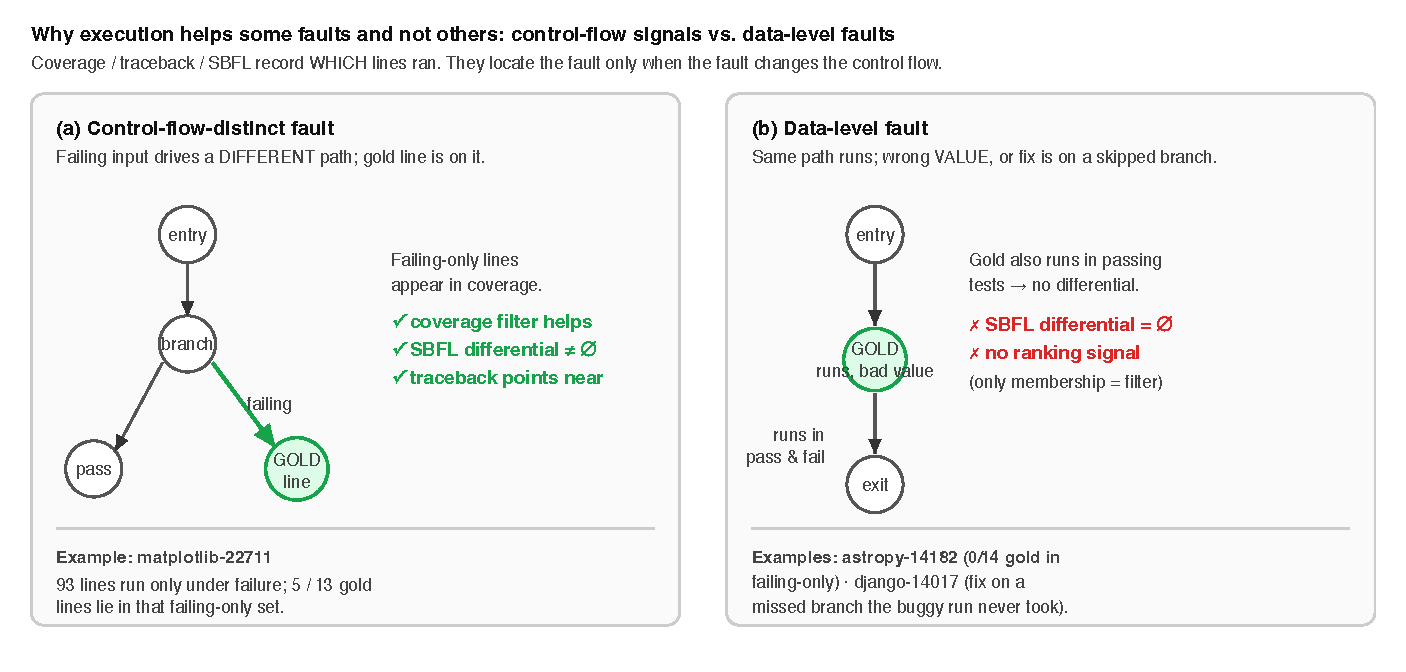
\includegraphics[width=\linewidth]{figures/fig2_taxonomy.pdf}
\caption*{\textbf{Figure 2.} The unifying distinction. (a) When the fault changes the control flow, the failing input drives a distinct path and the gold line appears in the failing-only coverage---coverage filter, SBFL differential, and traceback all fire (e.g., matplotlib-22711). (b) When the fault is data-level, the same lines run in passing and failing tests (so the SBFL differential is empty and there is no ranking signal---astropy-14182), or the fix lives on a branch the buggy run skipped (django-14017); coverage retains only \emph{membership}, i.e., a filter. SWE-bench instances appear dominated by case (b) (measured 6/9; proxy-extrapolated $\sim$66\%, indicative---\S7). This figure is the conceptual core of the paper (claim in RQ2.5, derivation in \S7).}
\end{figure}

% =====================================================================
\section*{6.\quad RQ3 --- Coverage-as-filter: the one use that works}

If coverage cannot \emph{rank} (RQ2.4) and is too coarse to \emph{be} the answer (RQ2.2), can it help at all? Yes---as a \textbf{filter} that \emph{narrows} the candidate set, but only where the gold is on the executed path. The filter raises recall (RQ3.1) and precision (RQ3.2) together, nothing finer beats it (RQ3.3), it survives the full LLM pipeline and four backbones (RQ3.4), and we delimit exactly when it applies (RQ3.5).

\smallskip\noindent\textbf{On-path scoping (and why it is mandatory).} We split instances into \emph{on-path} ($\ge$1 gold line executed) and \emph{off-path} (none, the 16\% of RQ2.3). The filter restricts candidates to executed lines; on-path the gold survives the filter, off-path it is \emph{deleted}. The split is therefore not a convenience---it is required for the filter to be sound. Note that on-path the gold is executed \emph{by construction}, so filtering to executed lines can only raise (never lower) R@$k$ and can only shrink the candidate set; the empirical content is thus the \emph{magnitude} of the gain and the on-path fraction (83\%), not its sign.

\smallskip\noindent\textbf{The on-path split is an oracle (deployability caveat).} On-path membership is defined via the gold lines, which a deployed localizer does not have, so the per-subset $+14$pp is an \emph{oracle-routed} figure, not a deployable one. Two gold-free policies bound the realizable gain on all crash bugs (from Table~4): \emph{always-filter} (no routing) yields $(57{\cdot}43.9+11{\cdot}0)/68=36.8$ vs.\ $32.3$ for pure static $={+}4.5$pp---the filter deletes the gold on the 16\% off-path---while perfect (oracle) routing yields $44.2={+}11.8$pp. A practical on-path \emph{detector} (e.g.\ traceback--region overlap) would land between these bounds; building one is future work. We therefore report the on-path contrast as the \emph{mechanism}, and $+4.5$pp as the current deployable floor. The same routing necessity holds at the \emph{full-pipeline} level across the three open backbones of Table~8: always-filter ranges $-3.0$ to $+8.8$pp on all crash (net-\emph{negative} on DeepSeek-V3.2, whose static off-path ranking is strong), whereas oracle routing is $+7.3$ to $+19.1$pp on all three---so on/off-path routing is mandatory beyond the def-use ranker, and a blind filter can hurt.

\subsection*{RQ3.1\quad Coverage-as-filter raises recall}
\begin{table}[t]
\centering\footnotesize
\caption*{\textbf{Table 4 --- Static def-use ranking vs.\ coverage-filter, four subsets (file-given, no LLM, \code{rq3/crash\_coverage\_rank\_test.py}).}}
\setlength{\tabcolsep}{4.5pt}
\begin{tabular}{lrrrrrrrrr}
\toprule
Subset & $n$ & A R@1 & B R@1 & A R@5 & B R@5 & A R@10 & B R@10 & A MRR & B MRR \\
\midrule
\textbf{crash\,$\cdot$\,on-path} & 57 & 10.5 & 14.0 & 28.1 & 29.8 & 29.8 & \textbf{43.9} & 0.184 & 0.244 \\
behavioral\,$\cdot$\,on-path & 131 & 10.7 & 13.0 & 22.9 & 26.7 & 27.5 & 34.4 & 0.169 & 0.210 \\
crash\,$\cdot$\,off-path & 11 & 18.2 & \textbf{0.0} & 45.5 & \textbf{0.0} & 45.5 & \textbf{0.0} & 0.283 & 0.000 \\
behavioral\,$\cdot$\,off-path & 40 & 5.0 & 0.0 & 25.0 & 0.0 & 35.0 & 0.0 & 0.163 & 0.000 \\
\bottomrule
\end{tabular}
\end{table}

The filter removes non-executed distractors while the (executed) gold survives, lifting it into the top-10: \textbf{+14.1pp R@10 on crash on-path} (29.8$\rightarrow$43.9; paired bootstrap 95\% CI $[3.5, 24.6]$) and +6.9pp on behavioral on-path---so the filter is an \emph{on-path}, crash-favored technique, not crash-exclusive. Off-path it is \textbf{catastrophic} ($\rightarrow$0), and crucially the \emph{static} ranker still scores 45.5 R@10 there: \textbf{static localization, not execution, must handle off-path bugs.} This dictates a routing design: filter on-path, fall back to pure static off-path.

\emph{Worked example (filter-rescue, django-16873).} The gold fix is in \code{defaultfilters.py} (982 LoC). The static def-use ranker scores \textbf{656} candidate lines and places the first gold line (589--591) at rank \textbf{\#40}---a miss at R@10. Restricting to the \textbf{75} lines the failing test actually executed (an 88\% cut) deletes the non-executed distractors that outranked the gold, lifting it to rank \textbf{\#6}---now a hit at R@10. Nothing about the ranker changed: the filter improves recall purely by removing structurally-irrelevant lines the static scorer could not otherwise rule out. This is the per-instance mechanism behind the aggregate +14pp, and it simultaneously shrinks the predicted set 8.7$\times$---recall and precision rising together on the same instance.

\begin{figure}[t]
\centering
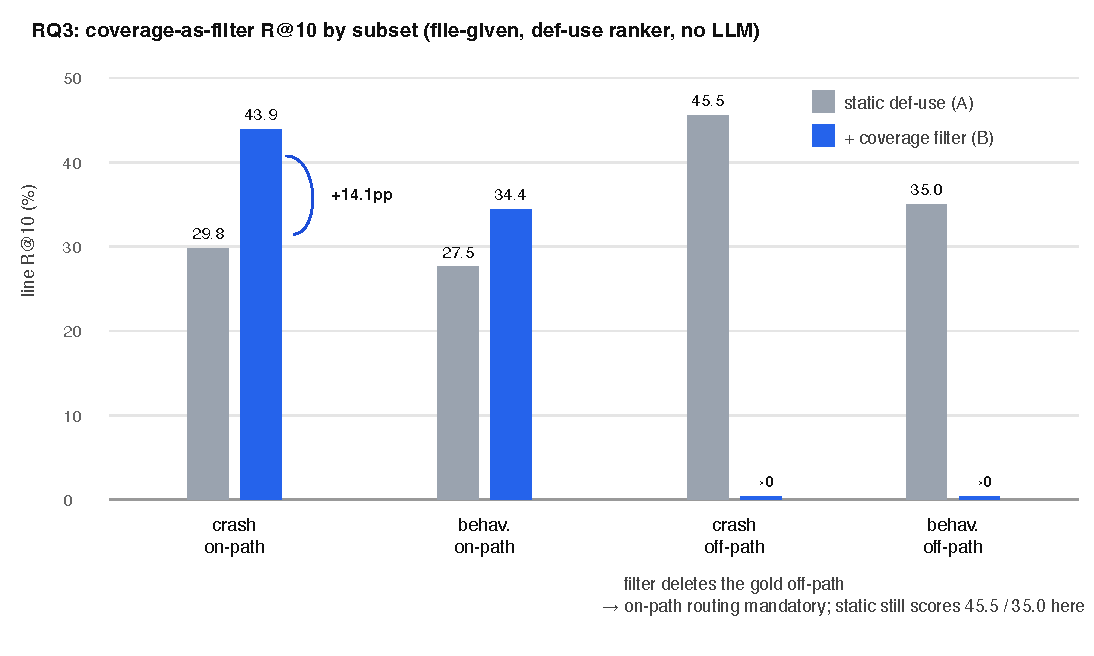
\includegraphics[width=0.86\linewidth]{figures/fig3_filter_result.pdf}
\caption*{\textbf{Figure 3.} Line R@10 by subset, static def-use (A) vs.\ + coverage filter (B). On-path the filter lifts recall (+14.1pp crash, +6.9pp behavioral); off-path it deletes the executed gold and collapses to 0---whereas the static ranker still scores 45.5/35.0---so on-path routing is mandatory.}
\end{figure}

\subsection*{RQ3.2\quad Coverage-as-filter also raises precision (resolves the wide-net)}
\begin{table}[t]
\centering\small
\caption*{\textbf{Table 5 --- Over-prediction width before/after the filter.}}
\setlength{\tabcolsep}{8pt}
\begin{tabular}{lrrr}
\toprule
Subset & candidate lines (static) & candidate lines (filter) & narrowing \\
\midrule
crash\,$\cdot$\,on-path & 837 & 378 & \textbf{$-$55\%} \\
behavioral\,$\cdot$\,on-path & 939 & 403 & $-$57\% \\
\bottomrule
\end{tabular}
\end{table}

The filter \textbf{halves the candidate set} \emph{while recall rises} (+14pp) and MRR improves (gold found at a better absolute rank, Table 4). The precision gain is in \emph{candidate-set width} (Table 5), directly fixing the ``spray a wide net, sacrifice precision to sustain recall'' behavior that RQ1's big-file precision wall (and prior wide-net localizers) exhibit; at the fixed top-10 deliverable, precision rises only modestly (e.g.\ $0.068\rightarrow0.084$ in the full pipeline, RQ3.4), so the win is in net width, not in top-$k$ precision. \emph{(EXAM as a fraction of candidates rises 0.177$\rightarrow$0.210---a real loss of rank-fraction efficiency from the shrinking denominator, not merely an artifact; we therefore claim a gain in \emph{absolute} first-gold rank (MRR) and candidate-set width, not in EXAM.)}

\subsection*{RQ3.3\quad What does \emph{not} work---ablations within the executed set}
\emph{Given the filter works, does any finer operation inside the executed set beat it? None does.} We tried four ways to do better than the plain filter inside the executed set; all fail, and the failures are informative.

\begin{table}[t]
\centering\small
\caption*{\textbf{Table 6 --- Candidate region quality on crash on-path ($n$=37, indicative): recall, median size, density=recall/size.}}
\setlength{\tabcolsep}{8pt}
\begin{tabular}{lrrr}
\toprule
Region & gold recall & median lines & density \\
\midrule
R1 = raw coverage & \textbf{100\%} & 325 & 0.31 \\
R2 = traceback functions $\cap$ coverage & 59.5\% & \textbf{23} & \textbf{2.59} \\
R3 = backward slice $\cap$ coverage & 59.5\% & 29 & 2.05 \\
R4 = R2 + 1-hop executed callees & 59.5\% & 25 & 2.38 \\
R5 = R2 + 2-hop executed callees & 62.2\% & 25 & 2.49 \\
Rall = all executed functions & 94.6\% & 279 & 0.34 \\
\bottomrule
\end{tabular}
\end{table}

\begin{itemize}
  \item \textbf{Traceback-only.} The gold is in a traceback function only 58\%, at the \emph{deepest} frame only 32\% (the root cause is upstream 68\% of the time), and it recovers only 19\% of the cases static misses (\code{rq2/crash\_fusion\_estimate.py})---a useful but bounded prior, not a solution.
  \item \textbf{Backward data-flow slice $\cap$ coverage (R3).} Identical recall to the traceback region (59.5\%) with \emph{more} lines---no gain; the off-stack root cause (in a function that already returned) is unreachable by an intraprocedural slice (\code{rq3/crash\_slice\_validation.py}).
  \item \textbf{Call-graph region expansion (R4/R5).} Adding 1-/2-hop executed callees of the traceback functions raises recall only 59.5$\rightarrow$59.5$\rightarrow$62.2\%; reaching high recall (Rall, 94.6\%) requires \emph{all} executed functions (279 lines)---back to the haystack (\code{rq3/crash\_region\_expand.py}). \textbf{There is no narrow, high-recall region for crash bugs}: R2 is high-density (2.59) but caps at $\sim$60\%; recall toward 100\% costs precision back.
  \item \textbf{SBFL.} The failing-vs-passing differential is bug-dependent and empty for data-level faults (RQ2.4, Table 3); it offers no usable narrowing here.
\end{itemize}

\subsection*{RQ3.4\quad The filter holds in the full vote+graph+LLM pipeline}
RQ3.1--3.3 isolate the coverage signal with the def-use ranker and no LLM. We now confirm the headline effect inside the \emph{full} pipeline---agentic region narrowing, $k$-sample self-consistency vote, and RRF ranking---on the frozen crash on-path subset ($n$=57, file-given, Qwen2.5-Coder-32B; \code{rq4/run\_all.py}). The pipeline realization of the filter is to \textbf{narrow the region shown to the vote to executed lines}, so the LLM votes within the executed set; we report a paired bootstrap 95\% CI over the per-instance hits. We compare four pipeline variants, each adding one component to the previous---\textbf{Static} (no coverage), \textbf{+score} (coverage added as an extra ranking score), \textbf{+filter} (the vote restricted to executed lines), and \textbf{+filter+score} (both)---plus two lower-bound anchors: the def-use slice and the self-consistency vote in isolation.

\begin{table}[t]
\centering\small
\caption*{\textbf{Table 7 --- Coverage in the full vote+graph+LLM pipeline (crash on-path, $n$=57, file-given, Qwen2.5-Coder-32B). (+filter+score) $-$ Static R@10 $=+12.3$pp, 95\% CI $[1.8, 22.8]$.}}
\setlength{\tabcolsep}{9pt}
\begin{tabular}{lrrr}
\toprule
Arm & R@1 & R@5 & R@10 \\
\midrule
\textbf{Static} \ no coverage & 29.8 & 50.9 & 56.1 \\
\textbf{+score} \ coverage added as a ranking score & 29.8 & 50.9 & 56.1 \\
\textbf{+filter} \ vote restricted to executed lines & 35.1 & 52.6 & \textbf{68.4} \\
\textbf{+filter+score} \ ($=$ +filter; score adds nothing) & 35.1 & 52.6 & \textbf{68.4} \\
\midrule
\emph{(lower-bound anchor)} def-use slice alone & 12.3 & 26.3 & 29.8 \\
\emph{(lower-bound anchor)} self-consistency vote alone & 31.6 & 47.4 & 56.1 \\
\bottomrule
\end{tabular}
\end{table}

The result mirrors the offline finding (Table 4) at the pipeline level: restricting the vote to executed lines (\textbf{+filter}$=$\textbf{+filter+score}) raises line R@10 from 56.1 to 68.4---\textbf{+12.3pp, 95\% CI $[1.8, 22.8]$, significant}---while \textbf{Static} and the coverage-\emph{score} variant (\textbf{+score}) are identical (56.1). That is, \textbf{the coverage \emph{score} term adds nothing; the gain comes entirely from narrowing the vote to executed lines}, exactly as the def-use ablation predicted (RQ2.4). (The score term's effect is \emph{exactly} zero at every $k$. An offline weight sweep rules out an under-weighting artifact: on the def-use ranker, blending the coverage score onto the filter leaves R@10 at 43.9 across weights $0.8$--$6.0\times$---identical to the pure filter---and onto the static ranker leaves R@10 at 29.8; the coverage score carries no ranking information at any weight.)

\begin{figure}[t]
\centering
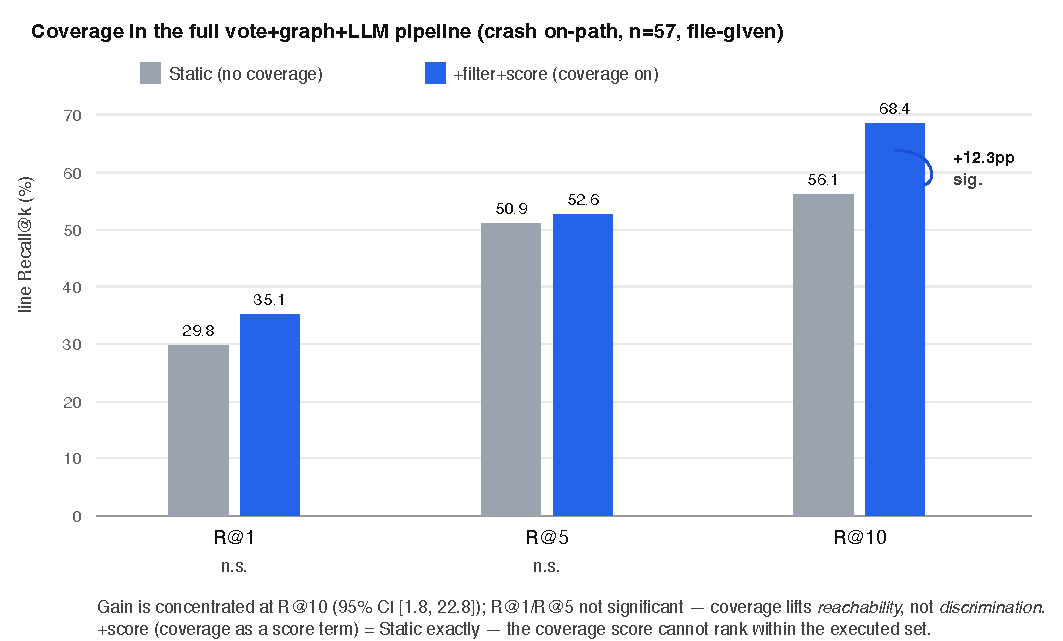
\includegraphics[width=0.84\linewidth]{figures/fig4_pipeline_result.pdf}
\caption*{\textbf{Figure 4.} Coverage in the full pipeline (crash on-path, $n$=57, file-given). The gain is concentrated at R@10 (+12.3pp, 95\% CI [1.8, 22.8], significant); R@1/R@5 are not significant. Coverage lifts \emph{reachability} (a gold line into the top-10), not \emph{discrimination} (ranking it first); the coverage \emph{score} term (+score) equals Static.}
\end{figure}

\smallskip\noindent\textbf{Reachability, not discrimination (Figure 4).} The gain is confined to R@10: R@1 ($+5.3$pp) and R@5 ($+1.8$pp) are \emph{not} significant, and fraction recall barely moves ($0.629\rightarrow0.644$, n.s.). Per instance, narrowing pulls the gold's first-hit rank from beyond-10 into the \emph{6--10} band (instances with the gold ranked 6--10 rise from 3 to 9), not into the top-5. Coverage thus lifts \emph{reachability}---getting a gold line into the top-10---but not \emph{discrimination}: among the $\sim$41 executed candidate lines the buggy line runs identically to its innocent neighbours, so the pipeline still cannot rank it first (precision $0.084$). This is the same ceiling self-consistency itself hits: the pipeline's vote surfaces the gold into the top-10 on 56\% of instances but ranks it first on only 30\% (Static, Table~7), and the coverage filter extends the \emph{same} axis---pushing R@10 to 68.4 while leaving R@1 statistically flat. Both buy reachability; neither buys discrimination. The effect is strongest on single-line fixes ($\Delta$R@10 $+18.2$pp, $\Delta$recall $+0.091$) and vanishes in fraction recall for multi-line fixes ($\Delta$recall $-0.002$). \emph{Caliber note:} these are \textbf{file-given} (oracle gold file) numbers and are \emph{not} comparable to ARISE's end-to-end results (which include file localization); the claim is the paired internal contrast Static vs.\ +filter+score on identical inputs.

\begin{table}[t]
\centering\small
\caption*{\textbf{Table 8 --- Cross-backbone replication of the coverage filter} ((+filter+score) $-$ Static; file-given S1, $n$=57, identical protocol; paired bootstrap 95\% CIs; \textbf{bold} = CI excludes 0). $\Delta$R@10 = reachability (primary endpoint); $\Delta$R@1 = discrimination; $\Delta$R@5 = intermediate band (\S3.3).}
\setlength{\tabcolsep}{3pt}\footnotesize
\begin{tabular}{lrrlll}
\toprule
Backbone & Static & +f+s & $\Delta$R@10 [CI] & $\Delta$R@5 [CI] & $\Delta$R@1 [CI] \\
\midrule
Qwen2.5-Coder-32B (paper) & 56.1 & 68.4 & \textbf{+12.3} [1.8, 22.8] & +1.8 [$-$10.5, 14.0] & +5.3 [$-$3.5, 14.0] \\
Qwen3.6-27B & 57.9 & 80.7 & \textbf{+22.8} [12.3, 35.1] & \textbf{+15.8} [3.5, 28.1] & +8.8 [$-$1.8, 19.3] \\
DeepSeek-V3.2 & 70.2 & 78.9 & \textbf{+8.8} [1.8, 17.5] & +8.8 [0.0, 17.5] & +0.0 [$-$10.5, 10.5] \\
GLM-4.5-Air & 50.9 & 59.6 & +8.8 [$-$3.5, 21.1] & \textbf{+17.5} [5.3, 29.8] & +1.8 [$-$10.5, 14.0] \\
\bottomrule
\end{tabular}
\end{table}

\smallskip\noindent\textbf{Cross-backbone replication (Table 8).} We re-ran the headline Static vs.\ +filter+score contrast on three further open backbones spanning distinct families and scales (file-given S1, $n$=57, identical protocol). \textbf{The filter gain replicates: $\Delta$R@10 is positive on all four backbones and significant on three}---Qwen2.5-Coder-32B $+12.3$, Qwen3.6-27B $+22.8$, DeepSeek-V3.2 $+8.8$pp (all 95\% CIs exclude 0); GLM-4.5-Air $+8.8$pp (CI $[-3.5,21.1]$, n.s.\ at this $n$, same point estimate as DeepSeek). Table~8 also reports the secondary endpoints, which sharpen the reachability/discrimination reading rather than qualify it away. At R@1---\emph{discrimination} under our operationalization (\S3.3)---the filter's gain is \textbf{not significant on any of the four backbones} (point estimates $0.0$ to $+8.8$pp; every 95\% CI includes 0): nowhere does narrowing the vote to executed lines significantly help rank the gold \emph{first}. The intermediate band R@5 is backbone-dependent: significant on Qwen3.6-27B ($+15.8$pp) and GLM-4.5-Air ($+17.5$pp), not on Qwen2.5-Coder-32B ($+1.8$pp) or DeepSeek-V3.2 ($+8.8$pp, CI $[0.0,17.5]$)---so on some backbones the filter does push the gold into the top-5, and the strict ``gain confined to R@10'' pattern of Figure~4 is Qwen2.5-Coder-specific. The two facts that replicate across all four backbones are exactly the title claim: reachability (R@10) gains are positive 4/4 and significant 3/4, and top-1 discrimination (R@1) never significantly moves.

\subsection*{RQ3.5\quad Conclusion (RQ3)}
Execution coverage's one robust contribution to crash-class line localization is a \textbf{filter} that, on the on-path subset, raises recall (+14pp R@10 with the def-use ranker; \textbf{+12.3pp in the full vote+graph+LLM pipeline}, significant, RQ3.4) and precision ($-$55\% candidates), and that must be \emph{routed} (on-path only). Within the executed set, every finer use fails: the SBFL differential is bug-dependent and empty for data-level faults, and slicing/region-expansion cannot produce a narrow high-recall region because the off-path/off-stack root causes are data-level. Crucially, the filter's R@1 (\emph{discrimination}) gain is significant on \emph{none} of the four backbones, while the intermediate R@5 band lifts significantly on two (Table 8)---so precise top-1 pinpointing still leans on the ranker (static def-use $+$ LLM) or a signal orthogonal to coverage. An \emph{assertion-rerank}---a coverage-orthogonal signal, \emph{not} a rung of the coverage ladder (Static / +score / +filter / +filter+score) above---lifts R@1/R@5 on two of three open backbones (Qwen3.6-27B $+7.0$/$+3.5$pp, GLM-4.5-Air $+8.0$/$+4.0$pp) but not DeepSeek-V3.2 and not significantly (M5$-$M4 paired deltas, $n{=}57/57/50$; protocol and full CIs in Appendix~A), so a coverage-orthogonal signal \emph{may} add discrimination, backbone-dependently---an exploratory observation, not a confirmed effect. Cross-backbone replication confirms the headline: $\Delta$R@10 is positive on all four backbones tested and significant on three (Table 8).

% =====================================================================
\section*{7.\quad Discussion --- Control-flow vs.\ data-level faults}

A single distinction organizes every result above. The organizing claim is stated in RQ2.5; here we derive each result from it and draw out its consequences.

\smallskip\noindent\textbf{The taxonomy (Figure 2).} Execution coverage, traceback, and SBFL are all \textbf{control-flow} signals: they tell you \emph{which lines ran} and \emph{in what order}. They are powerful exactly when the bug changes the control flow---a crash that takes a distinct path (matplotlib-22711), the crash-oriented bugs of Defects4J~\citep{defects4j} on which SBFL was validated. But SWE-bench issues appear dominated by \textbf{data-level} faults---where the failing-vs-passing differential is computable, 6 of 9 instances (67\%, Wilson 95\% CI $35$--$88\%$) are data-level (gold absent from the failing-only set), the other 3 being the control-flow-distinct matplotlib cases of Table~3. A patch-structure proxy---counting a fix control-flow-distinct when it adds a substantively-bodied branch, else data-level (guard and insertion fixes are data-level, per the mechanism above)---was \emph{calibrated in-sample} on these 9 (8/9 agreement; a naive branch-adding rule scores only 4/9). Applied to all 300 instances it estimates a data-level \emph{majority}---66\% under the calibrated rule, 49\% under the naive one (\code{rq3/datalevel\_classifier.py})---an indicative extrapolation consistent with the coverage-based 67\%, not an independent measurement. The direct $n{=}9$ measurement alone does not establish a majority (its CI crosses 50\%); the majority claim rests on the proxy extrapolation plus the mechanism below, and we mark it \emph{indicative} wherever it is used. The mechanism is the same throughout: the buggy line \emph{runs} and produces a \emph{wrong value} (which passing tests also execute, RQ2.4), or the bug is a \emph{wrong branch condition} so the fix line is on the path that \emph{should} have run (RQ2.3). For data-level faults, control-flow signals are structurally blind.

\smallskip\noindent\textbf{Why each result follows.} (i) Coverage barely separates crash from behavioral (RQ2.2) because most crash bugs are still data-level on shared paths. (ii) The 83\% ceiling (RQ2.3) is the missed-branch (data-level control fault) plus insertions. (iii) SBFL's differential is empty for data-level bugs and only coarsely present for the control-flow-distinct minority (RQ2.4). (iv) The \emph{only} thing coverage robustly provides---membership (``this line ran'')---is a pure \emph{filter}, which is exactly what RQ3 exploits.

\smallskip\noindent\textbf{Implication for ``execution-grounded'' localization.} Our results bound the 2026 execution-grounding wave at line granularity: execution coverage is a recall-side \emph{filter}, not a ranking signal, and its value is confined to the on-path subset. Methods that use coverage to \emph{rank} (raw SBFL) or as a \emph{direct} candidate set will not beat strong static localizers on SWE-bench; the productive design is coverage-as-filter + a strong static/LLM ranker, with on/off-path routing. This bound is on \emph{coverage- and spectrum-based} signals; execution signals that capture value flow (mutation, value/state tracing, taint) could in principle reach data-level faults and are untested here.

\smallskip\noindent\textbf{Why discrimination is the hard axis.} The reachability/discrimination split (RQ3.4) shares a cause with the generator--verifier asymmetry familiar from LLM reasoning~\citep{cannot_self_correct,verifiers}. The pipeline's ranking is produced by self-consistency---the model verifying its own samples---and the signals available to it (vote counts, coverage \emph{membership}, def-use adjacency) are all \emph{co-sourced} with the candidate set: they certify that a line was reached but carry no information separating the buggy line from its executed neighbours. This is why the coverage \emph{score} term adds exactly nothing (+score$\equiv$Static, RQ3.4) even as the coverage \emph{filter} helps---filtering is a membership operation, whereas scoring would require discrimination the signal does not contain. Consistent with this, the one lever that \emph{does} move R@1/R@5---an assertion-grounded rerank keyed off the failing test's expected-vs-observed values (RQ3.5; protocol in Appendix~A)---is \emph{orthogonal} to both coverage and the model's own vote, and it helps backbone-dependently. (What follows, including Table~9(a), is an \emph{exploratory, RQ4-facing} probe---an upper bound and a first deployable step---not part of the confirmatory RQ2/RQ3 package.) To test whether the ceiling is intrinsic to the task or merely an artifact of \emph{same-model} self-consistency, we upper-bound what a \emph{heterogeneous, stronger} verifier could recover: on S1 we take, per instance, the \emph{oracle union} of the base backbone and a stronger heterogeneous model (DeepSeek-V3.2)---counting a hit@$k$ if \emph{either} surfaces a gold line in the top-$k$ (\code{rq4/m\_hetero\_upper.py}). This lifts R@1 from $35.1$ to $49.1$ ($+14.0$pp, paired bootstrap 95\% CI $[5.3,22.8]$), R@5 by $+17.6$pp $[8.8,28.1]$, and R@10 by $+19.3$pp $[10.5,29.8]$---all significant. The discrimination ceiling is therefore \emph{not intrinsic to same-model self-consistency}: on the very instances the base ranks the gold low, a heterogeneous, orthogonal signal recovers it. This is an oracle-union \emph{upper bound}, not a deployable gain. To see how much a \emph{real} verifier realizes, we ran DeepSeek-V3.2 as a deployable re-ranker of the same candidate set---given only the issue and the candidate code, no gold (\code{rq4/m\_hetero\_real.py})---which recovers roughly half the bound: R@1 $35.1\rightarrow42.1$ ($+7.0$pp), R@5 $52.6\rightarrow64.9$ ($+12.3$pp), R@10 $68.4\rightarrow77.2$ ($+8.8$pp), positive on all three but \emph{not} significant at $n{=}57$ (Table~9). A heterogeneous verifier thus realizes part of the recoverable discrimination \emph{without} the gold; closing the gap to the oracle bound---and doing so cheaply---is future work (RQ4, \S9).

\begin{table}[t]
\centering\small
\caption*{\textbf{Table 9 --- Recovering discrimination beyond same-model self-consistency} (S1 crash on-path, $n$=57, file-given; panel (a) is \emph{exploratory, RQ4-facing}), and data-level prevalence at dataset scale.}
\setlength{\tabcolsep}{7pt}
\begin{tabular}{lrrr}
\toprule
\multicolumn{4}{l}{\emph{(a) Ranker / bound on the coverage-filtered candidate set --- line R@$k$}}\\
 & R@1 & R@5 & R@10 \\
\midrule
Base: Qwen2.5-Coder-32B, +filter+score (self-consistency) & 35.1 & 52.6 & 68.4 \\
$+$ DeepSeek-V3.2 verifier re-rank (deployable, no gold) & 42.1 & 64.9 & 77.2 \\
\quad{\footnotesize $\Delta$ vs base $+7.0$/$+12.3$/$+8.8$pp, n.s.\ at $n$=57} & & & \\
Oracle union $\oplus$ DeepSeek-V3.2 (\emph{upper bound}) & \textbf{49.1} & \textbf{70.2} & \textbf{87.7} \\
\quad{\footnotesize $\Delta$ vs base $+14.0$/$+17.6$/$+19.3$pp, all sig.} & & & \\
Oracle union, best of 4 backbones (\emph{upper bound}) & 56.1 & 75.4 & 87.7 \\
\midrule
\multicolumn{4}{l}{\emph{(b) Data-level proportion (patch proxy, all 300; in-sample calibrated)}}\\
Rule & DL\% & \multicolumn{2}{r}{Wilson (sampling)} \\
\midrule
calibrated (in-sample 8/9) & 66 & \multicolumn{2}{r}{61--71} \\
naive branch-adding (4/9) & 49 & \multicolumn{2}{r}{43--54} \\
\bottomrule
\end{tabular}
\end{table}

\smallskip\noindent\textbf{Relation to classical SBFL.} Our SBFL finding does \emph{not} contradict decades of SBFL success on Defects4J---it delimits it. SBFL works where bugs are control-flow-distinct and test suites isolate them; the matplotlib cases (Table 3) confirm the mechanism still fires when those conditions hold. SWE-bench simply violates the conditions for most instances.

% =====================================================================
\section*{8.\quad Threats to Validity / Limitations}
\begin{itemize}
  \item \textbf{Construct (offline ranker).} The def-use-only RQ2/RQ3 experiments are file-given without an LLM to isolate the coverage signal; the headline filter effect is confirmed inside the full vote+graph+LLM pipeline (RQ3.4: +12.3pp R@10, $n$=57, Qwen2.5-Coder-32B) and \emph{replicates across four backbones} (Table 8: $\Delta$R@10 positive on 4/4, significant on 3/4).
  \item \textbf{Construct (reproduction-test oracle).} The filter requires the \emph{gold} failing test to exist and execute in Docker to produce coverage; on a fresh issue that test must first be generated (an open problem), and per-instance Docker execution is costly relative to the on-path-only gain. Our numbers therefore assume an oracle reproduction test. Relatedly, the on/off-path \emph{routing} is defined via gold lines (\S6); a deployable system needs a gold-free on-path detector, and the realizable un-routed gain on all crash bugs is $+4.5$pp (vs.\ the $+14$pp oracle-routed on-path contrast).
  \item \textbf{Internal (sample sizes).} Several effects rest on modest $n$ and are reported without confidence intervals; these should be read as \emph{indicative}: the SBFL differential (Table 3) is $n$=9 over 4 repos (the per-repo pattern---matplotlib positive, astropy/sklearn/seaborn null---is striking, and a patch-structure proxy calibrated in-sample on these 9 gives an indicative data-level majority ($\sim$66\%) over all 300 (\S7), though the coverage-based \emph{measurement} remains $n$=9: 6/9 data-level, Wilson 95\% CI $35$--$88\%$, consistent with but not by itself establishing a majority); the off-path subset is $n$=11; the region-quality ablation (Table 6) is $n$=37; and several Table 1 domain/size strata are $n\le23$ (scikit-learn, matplotlib, sphinx). The two load-bearing effects \emph{do} carry paired bootstrap 95\% CIs---the def-use coverage-filter (+14pp, $n$=57 crash on-path) and the full-pipeline confirmation (+12.3pp, RQ3.4, $n$=57). We designate \textbf{R@10 the a-priori primary endpoint} (it operationalizes \emph{reachability}, the quantity the filter can affect) and treat R@1 (\emph{discrimination}) and R@5 (intermediate band) as secondary, exploratory endpoints; this pre-specification, rather than a post-hoc correction, is why we report R@10 as the confirmatory result and read the reachability-not-discrimination pattern as exploratory. Both load-bearing CIs nonetheless have lower bounds near zero (offline $[3.5,24.6]$, pipeline $[1.8,22.8]$), so the effect \emph{size} is established only loosely; the cross-backbone replication (Table~8: $\Delta$R@10 positive on 4/4 backbones, significant on 3/4) is our primary evidence that the \emph{sign} of the effect is real.
  \item \textbf{Internal (bug-type classifier), now validated.} Crash/behavioral and on/off-path were assigned by a regex proxy over issue text and tests, then re-checked against the \emph{actual} FAIL\_TO\_PASS traceback collected in Docker for the full crash subset ($n$=68): \textbf{on/off-path agreed 68/68 (zero flips)}, and the crash label held on 25/26 cleanly-classified instances. The frozen S1 main set is unchanged, so the headline rests on correctly-labeled instances.
  \item \textbf{External (single benchmark / language).} Results are SWE-bench-Lite, Python. On crash-oriented C benchmarks or Defects4J~\citep{defects4j}, where bugs are more control-flow-distinct, SBFL may well help---an explicit, mechanism-predicted boundary (a conjecture we do not test here), not a contradiction.
  \item \textbf{Collection coverage.} SBFL collection skips Django (non-pytest \code{PASS\_TO\_PASS} names); a three-instance SymPy collection attempt returned empty coverage and is excluded as no-data (\S3.4); cross-repo claims span astropy/matplotlib/scikit-learn/seaborn only.
\end{itemize}

% =====================================================================
\section*{9.\quad Conclusion and Future Work (RQ4)}

We asked when execution grounding helps LLM line-level localization \emph{beyond} the model's own self-consistency. We first mapped \emph{why} localization fails (RQ1: file gate, file size, domain, multi-file), then \emph{falsified} execution coverage as a direct localization signal with a three-part mechanistic root cause (RQ2: coarseness, an 83\% structural ceiling from off-path fixes, a bug-dependent SBFL differential present only for control-flow-distinct faults), and showed that the \emph{one} effective use of coverage is a \textbf{filter} that raises recall (+14pp, an oracle-routed contrast; the deployable un-routed floor is $+4.5$pp) and precision ($-$55\% candidates) on the on-path crash subset, replicated across four backbones (significant on three), with a sharp on/off-path boundary (RQ3). The unifying finding is a signal typology: both self-consistency and execution coverage are \emph{membership} signals that certify \emph{reachability}, and neither adds \emph{discrimination}---the filter's R@1 gain is significant on none of the four backbones---because SWE-bench faults appear predominantly \emph{data-level} (measured 6/9; proxy-extrapolated $\sim$66\%, indicative)---the buggy line runs identically to its executed neighbours. Not every external signal helps an LLM equally: a signal that only certifies reachability cannot break a discrimination ceiling. This bounds \emph{coverage- and spectrum-based} line localization; richer execution signals (mutation, value/state tracing) are untested.

\smallskip\noindent\textbf{RQ4 (future).} If reachability is saturated but discrimination is the wall, the open question is what signal breaks it. Our typology points away from anything co-sourced with the candidate set and toward signals \emph{orthogonal} to coverage and to same-model self-consistency: a failing test's expected-vs-observed values (the assertion-rerank of RQ3.5 is a first, backbone-dependent step), or a \emph{heterogeneous, stronger} verifier. We both \emph{upper-bound} and take a first \emph{deployable} step at the latter (\S7, Table~9): the per-instance oracle union of the base and a stronger heterogeneous model lifts R@1 to $49.1$ ($+14.0$pp, significant), and a real DeepSeek-V3.2 verifier re-ranking the same candidates \emph{without} the gold reaches $42.1$ ($+7.0$pp, n.s.\ at $n{=}57$)---realizing about half the bound. So the discrimination the filter cannot supply \emph{is} recoverable, in principle fully and in practice partly, from a signal orthogonal to same-model self-consistency. Converting that oracle bound into a \emph{deployable} verifier---one that picks without the gold, routed against the static handling off-path bugs require---is the natural next step, reserved here so the present characterization stands independent of that harder goal.

% =====================================================================
\bibliographystyle{unsrt}   % 纯数字、按出现顺序；避免占位条目无作者时的 natexlab 标号残留
\bibliography{refs}

% =====================================================================
\section*{Appendix A --- Assertion-rerank (M5) protocol (exploratory)}

\noindent\textbf{Substrate and scope.} M5 operates on the output of the coverage-filtered pipeline arm (+filter+score, \S6): the ranked list of candidate lines for the gold file, on the frozen S1 crash on-path subset. It is a single, focused LLM call per instance that re-orders \emph{only the top-10 head} of that ranking; the tail is preserved unchanged.

\smallskip\noindent\textbf{Evidence extraction (no LLM).} The ``expected-vs-observed'' evidence is extracted deterministically (\code{test\_evidence.py}): (i) the failing test name(s) from \code{FAIL\_TO\_PASS}; (ii) the assertion lines of that test from the instance's test patch; (iii) the observed traceback/error quoted in the issue text. The three parts are concatenated and truncated to 1{,}600 characters. If no usable evidence is found, M5 is the identity (the input ranking is returned).

\smallskip\noindent\textbf{The call.} One completion at temperature $0.0$ (\code{region\_loc.py::assertion\_rerank}). The prompt contains the issue summary (truncated to 3{,}500 characters), the evidence block, and the ten candidates, each shown with $\pm$2 lines of context; the instruction asks the model to reason \emph{backward} from the observed failure to the line(s) that \emph{produce} the wrong value/behavior (root cause), and to output only line numbers drawn from the candidates, most-likely first. Parsed picks are placed first, followed by unpicked head lines in their original order, then the untouched tail; on a parse failure or API error the input ranking is returned unchanged. The re-rank therefore permutes the top-10 set but never alters its membership.

\smallskip\noindent\textbf{Evaluation.} M5 is evaluated as its own pipeline pass (driver \code{rq4/run\_all.py}, M5 arm; results \code{rq4/results/t3t6\_cross\_backbone.json}), paired per instance against the +filter+score pass; because each pass redraws the self-consistency vote, small R@10 differences reflect vote resampling, while the rerank itself only permutes the top-10 head. Paired bootstrap 95\% CIs, same procedure as Table~8. M5 was run on the three open API backbones (not on the paper's Qwen2.5-Coder-32B, which our API provider does not serve); for GLM-4.5-Air, 7 of 57 instances lacked an evaluable M5 arm (call failures) and are excluded pairwise, leaving $n{=}50$.

\begin{center}\small
\begin{tabular}{lrlll}
\toprule
Backbone & $n$ & $\Delta$R@1 [CI] & $\Delta$R@5 [CI] & $\Delta$R@10 [CI] \\
\midrule
Qwen3.6-27B & 57 & +7.0 [$-$3.5, 17.5] & +3.5 [$-$3.5, 10.5] & $-$1.8 [$-$7.0, 3.5] \\
DeepSeek-V3.2 & 57 & $-$1.8 [$-$14.0, 10.5] & $-$3.5 [$-$14.0, 5.3] & $-$3.5 [$-$10.5, 3.5] \\
GLM-4.5-Air & 50 & +8.0 [$-$4.0, 20.0] & +4.0 [$-$8.0, 16.0] & +2.0 [$-$12.0, 16.0] \\
\bottomrule
\end{tabular}
\end{center}

\noindent All M5$-$M4 deltas are non-significant (every CI includes 0); we accordingly present M5 only as an exploratory, RQ4-facing probe of a coverage-orthogonal signal (RQ3.5, \S7), not as a confirmed effect.

% =====================================================================
\section*{Appendix B --- Table 2 provenance (illustrative DeepSeek-V3 runs)}

\noindent\textbf{Common setup.} All three rows use \code{deepseek-ai/DeepSeek-V3}~\citep{deepseekv3} through an OpenAI-compatible API, on \textbf{SWE-bench Verified} (a different dataset and backbone from the paper's main experiments---hence \emph{illustrative} and never compared with them). Instances are drawn from the Verified pool after a deterministic seed-0 shuffle (repo diversity); per-instance records, prompts' input fields, and all summary statistics ship in the artifact (\code{archive/p0\_openai\_deepseek\_v3.json}, \code{p1\_...}, \code{p2\_...}), and the drivers for rows 1--2 are \code{p0\_line\_recall.py} and \code{p1\_realistic.py}.

\smallskip\noindent\textbf{Row 1 (single-file, file given; $n{=}40$).} The first 40 instances (after the shuffle) whose gold patch edits exactly one Python file of $\le$500 lines (empirical range 48--490). The model sees the full numbered file plus the issue and predicts the decisive lines/ranges. \textbf{(exact)} $=$ mean per-instance fraction of gold edit-region lines exactly matched by the predicted line numbers ($0.584$); \textbf{over-prediction} $=$ mean ratio of predicted lines to gold lines ($2.85\times$).

\smallskip\noindent\textbf{Row 2 (realistic two-stage; $n{=}40$).} File \emph{not} given: stage 1 shows the issue plus the repository's full Python file list and asks for top-5 suspect files (\textbf{file hit@5} $=0.90$); stage 2 runs the row-1 line prompt on the gold file when it was found. \textbf{e2e} line recall counts a file miss as 0 ($0.528$); \textbf{given-found} conditions on the file being found ($0.587$).

\smallskip\noindent\textbf{Row 3 (multi-file; $n{=}20$).} Instances whose gold patch spans $\ge$2 files (mean 2.45 gold files). \textbf{all-gold-files-found} $=$ fraction of instances where every gold file appears in the predicted file set ($0.35$); \textbf{global line recall} $=$ gold lines recovered over \emph{all} gold files ($0.277$). The stage-1/stage-2 protocol matches row 2. (The row-3 driver script has been superseded; the artifact retains the complete per-instance records and summary from which Table~2 is reproduced.)

\end{document}
